\documentclass[manuscript,review,anonymous]{acmart}

\citestyle{acmauthoryear}

\begin{document}

\title{Non-Directional Pre-Disclosure Drift Under Fair Disclosure: Evidence from Korean Earnings Announcements}

\author{Yongjun Kim}
\email{yjkim0123@ajou.ac.kr}
\orcid{0000-0003-4234-4883}
\affiliation{%
  \institution{Ajou University}
  \department{Department of Software}
  \city{Suwon}
  \country{South Korea}
}

\begin{abstract}
Does South Korea's Fair Disclosure regulation effectively ensure that earnings information reaches all market participants simultaneously? Using 2,221 earnings disclosure filings from 64 KOSPI-listed companies across 12 chaebol groups (2020--2026), we find that pre-disclosure abnormal returns, while statistically significant under parametric tests (CAR[-5,$-$1] = +0.52\%, $p$<0.001), do not predict the direction of actual earnings surprises (49.0\% accuracy, $p$=0.649; Spearman $\rho$=$-$0.006, $p$=0.876). Non-parametric tests confirm that the drift is driven by outliers rather than systematic directional movement (sign test $p$=0.585; Wilcoxon $p$=0.142). In contrast, the first post-disclosure trading day (Day +1) responds sharply and correctly to earnings surprises: positive surprises generate AR of +0.55\%, negative surprises $-$0.58\% ($p$<0.001), with 60.6\% direction accuracy ($p$<0.001). We further document that 96.5\% of filings occur after market close, making Day 0 effectively pre-disclosure. These results are robust to firm-clustered and month-clustered standard errors. Our findings suggest that Korea's Fair Disclosure regime effectively prevents directional information leakage, even though non-directional price noise and abnormal volume emerge in the pre-disclosure period.
\end{abstract}

\begin{CCSXML}
<ccs2012>
<concept>
<concept_id>10002951.10003317.10003347.10003350</concept_id>
<concept_desc>Information systems~Online analytical processing</concept_desc>
<concept_significance>500</concept_significance>
</concept>
<concept>
<concept_id>10002951.10003260.10003282</concept_id>
<concept_desc>Information systems~Data analytics</concept_desc>
<concept_significance>500</concept_significance>
</concept>
</ccs2012>
\end{CCSXML}

\ccsdesc[500]{Information systems~Online analytical processing}
\ccsdesc[500]{Information systems~Data analytics}

\keywords{Fair disclosure, Earnings announcements, Pre-announcement drift, DART, Korean stock market, Event study, Market efficiency, Earnings surprise}

\maketitle

\section{Introduction}

Pre-announcement drift in stock prices is a well-documented phenomenon across global equity markets \cite{kaniel2012individual}. When stock prices move before official earnings announcements, a natural concern arises: is material information leaking to select market participants in violation of fair disclosure regulations? This concern motivates securities regulators worldwide to mandate simultaneous public dissemination of material information.

South Korea implemented its Fair Disclosure regulation in November 2002, requiring listed companies to disclose material information simultaneously to all market participants through the DART (Data Analysis, Retrieval and Transfer) electronic filing system. While early studies found evidence of improved disclosure environments following the regulation's adoption \cite{yun2012fair, park2020disclosure}, whether the regulation continues to be effective over two decades later remains an open question.

This study examines the long-term effectiveness of Korea's Fair Disclosure regulation by analyzing 2,221 earnings disclosure filings from 64 major KOSPI-listed companies between 2020 and 2026. Our approach differs from prior work in a critical respect: rather than simply documenting the existence of pre-disclosure price movement, we test whether such movement is \textit{directionally informative}---that is, whether it predicts the sign of the actual earnings surprise.

Our findings reveal an important pattern. We observe statistically significant pre-disclosure abnormal returns under standard parametric tests (CAR[-5,$-$1] = +0.52\%, $p$<0.001 under the market model; $p$=0.032 with month-clustered standard errors). However, this drift bears no systematic relationship to the direction of actual earnings surprises. Pre-disclosure returns predict surprise direction with only 49.0\% accuracy---no better than a coin flip ($p$=0.649). Non-parametric tests (sign test, Wilcoxon signed-rank) fail to confirm the parametric result, indicating that the observed mean drift is driven by outliers rather than a pervasive pattern.

In contrast, the market responds sharply and correctly to the actual earnings news on the disclosure date. Positive earnings surprises generate a CAR[0,+1] of +0.81\%, while negative surprises generate $-$0.47\%, a highly significant difference ($p$<0.001). This finding is consistent with effective Fair Disclosure: material information is incorporated into prices only when it becomes publicly available.

We make four contributions. First, we provide the first long-term assessment of Korea's Fair Disclosure regime using recent data spanning the COVID-19 and post-pandemic periods. Second, we demonstrate the critical distinction between the \textit{existence} of pre-disclosure drift (which is ubiquitous) and its \textit{directional informativeness} (which would indicate information leakage). Third, we document a previously overlooked institutional feature---96.5\% of DART fair disclosure filings are submitted after market close---that has important implications for event study interpretation. Fourth, we provide cross-sectional and temporal analyses that reveal significant heterogeneity across chaebol groups, fiscal quarters, and years.

\section{Literature Review}

\subsection{Fair Disclosure Regulation}

Fair disclosure regulation addresses selective disclosure, whereby corporate insiders share material information with favored market participants before public release \cite{heflin2003regulation}. In the U.S., Regulation Fair Disclosure (Reg FD), implemented in 2000, produced mixed evidence: \citet{ahmed2003impact} find reduced information asymmetry, while \citet{heflin2003regulation} document reduced information quality. \citet{bailey2003regulation} provide comprehensive evidence on market, analyst, and corporate responses to Reg FD, and \citet{eleswarapu2004impact} document reduced information asymmetry and trading costs following implementation. \citet{gomes2007sec} further show that Reg FD affected the cost of capital, particularly for smaller firms.

In Korea, \citet{yun2012fair} examined the effect of fair disclosure regulation on the timeliness and informativeness of earnings announcements, while \citet{park2020disclosure} investigated how disclosure frequency under the regulation affects the information environment and cost of capital. \citet{yoon2011impact} provide early evidence on the impact of fair disclosure on the Korean stock market, and \citet{lee2012testing} test regulatory effectiveness using Korean data in an emerging market context. However, these studies do not examine whether pre-disclosure price movements are directionally informative with respect to the actual earnings news---the central question of our study.

\subsection{Pre-Announcement Drift and Its Interpretation}

Pre-announcement drift in stock prices is well-documented but its interpretation is debated. \citet{meulbroek1992comparison} provides evidence of illegal insider trading preceding announcements. \citet{bernile2016can} show that informed trading occurs even ahead of macro-news announcements where information is tightly controlled. However, \citet{kaniel2012individual} demonstrate that individual investor trading patterns around earnings announcements can generate drift without requiring illegal information leakage.

Critically, the mere existence of pre-announcement drift does not establish information leakage. Predictable earnings patterns allow sophisticated investors to position ahead of announcements through legal means \cite{atiase1985predisclosure}. \citet{chae2005trading} shows that abnormal volume before announcements reflects information asymmetry but may arise from varying levels of investor sophistication rather than illegal tip-offs. A related literature on post-earnings-announcement drift (PEAD) demonstrates that markets may take days or weeks to fully incorporate earnings information \cite{bernard1989post}, further complicating the interpretation of short-window event studies.

\subsection{Event Study Methodology}

The standard event study framework \cite{brown1985using, mackinlay1997event} relies on parametric tests of mean abnormal returns. However, \citet{kolari2010event} demonstrate that cross-sectional correlation of abnormal returns can substantially inflate test statistics, particularly when events cluster in calendar time. We incorporate both non-parametric alternatives and standardized returns to address these concerns.

\subsection{Korean Market Context}

The Korean stock market features concentrated chaebol ownership, a mandatory electronic disclosure system (DART), significant retail investor participation, and relatively strict insider trading regulations. \citet{beny2005impact} demonstrates that stronger insider trading enforcement is associated with more efficient stock prices across countries, providing cross-country evidence relevant to our Korean setting. These institutional features, combined with the comprehensive DART database, make Korea an ideal setting for testing fair disclosure effectiveness.

\section{Data and Methodology}

\subsection{Data Sources}

We collect all Fair Disclosure of Operating Results filings from DART between January 2020 and March 2026 using the OpenDartReader API. We focus on original filings, excluding corrections. Our sample comprises 2,221 disclosures from 64 companies across 12 chaebol groups: Samsung (12), Hyundai Motor (8), LG (8), SK (7), HD Hyundai (5), Hanwha (5), POSCO (4), Lotte (4), Doosan (4), CJ (3), KT (2), and GS (2). Daily stock price and volume data are obtained from FinanceDataReader.

\subsection{Filing Time Classification}

We classify filing times using the DART receipt number prefix. In our sample, 96.5\% of earnings disclosures carry the ``800'' prefix, indicating filing after the 15:30 KST market close. This has fundamental implications: for these filings, the Day~0 return is entirely pre-disclosure, and the first trading day where the market can react is Day~+1.

\subsection{Market Model}

We employ the market model with a [-250,$-$30] estimation window \cite{mackinlay1997event}:
\begin{equation}
R_{i,t} = \alpha_i + \beta_i R_{m,t} + \epsilon_{i,t}
\end{equation}
where $R_{m,t}$ is the KOSPI index return. We require a minimum of 60 trading days in the estimation window, yielding 2,208 events with valid estimates. The average estimated beta is 0.978. For robustness, we also report market-adjusted returns ($\alpha=0$, $\beta=1$).

\subsection{Earnings Surprise Measure}

We extract year-over-year (YoY) operating profit changes from the disclosure texts. Events where YoY operating profit increases are classified as positive surprises; decreases as negative surprises. Of the 2,208 events with valid market model estimates, 584 have parseable earnings surprise data: 358 positive and 226 negative surprises; unparseable cases primarily involve missing comparative periods, newly listed firms, or format variations in disclosure texts.

We acknowledge that the standard measure in earnings announcement studies is the analyst consensus forecast surprise \cite{livnat2006comparing}. However, comprehensive analyst consensus data for Korean firms are not freely available for our full sample period, and commercial databases require institutional subscriptions. The YoY operating profit change, while crude, captures the directional content of the earnings news and provides a conservative test.

\subsection{Statistical Tests}

We report multiple test statistics to ensure robustness: parametric cross-sectional $t$-tests, non-parametric tests (binomial sign test, Wilcoxon signed-rank), and standardized abnormal returns. We also report firm-clustered and month-clustered standard errors to address cross-sectional dependence \cite{kolari2010event}.

\section{Empirical Results}

\subsection{Pre-Disclosure Returns: Significant but Non-Directional}

Table~\ref{tab:ar} presents daily abnormal returns. Parametric $t$-tests indicate significant positive returns on several pre-disclosure days, particularly Day~$-$1 (+0.256\%, $t$=4.57). However, the sign test reveals that only 48--50\% of individual returns are positive on each pre-disclosure day---no better than chance.

\begin{table}[h]
\caption{Daily Abnormal Returns: Parametric vs.\ Non-Parametric Tests}
\label{tab:ar}
\begin{tabular}{lrrrrrrr}
\toprule
& & \multicolumn{2}{c}{Parametric} & \multicolumn{2}{c}{Sign Test} & \multicolumn{2}{c}{Standardized} \\
\cmidrule(lr){3-4} \cmidrule(lr){5-6} \cmidrule(lr){7-8}
Day & AR (\%) & $t$ & $p$ & \% Pos & $p$ & SAR & $p$ \\
\midrule
$-$5 & 0.101 & 2.09 & 0.037 & 50.5 & 0.609 & 0.040 & 0.048 \\
$-$4 & 0.071 & 1.50 & 0.134 & 49.8 & 0.930 & 0.041 & 0.043 \\
$-$3 & 0.086 & 1.71 & 0.088 & 49.3 & 0.562 & 0.022 & 0.279 \\
$-$2 & 0.006 & 0.14 & 0.888 & 48.9 & 0.295 & $-$0.002 & 0.935 \\
$-$1 & 0.256 & 4.57 & $<$0.001 & 50.1 & 0.909 & 0.089 & $<$0.001 \\
\midrule
0 & 0.141 & 2.00 & 0.046 & 49.8 & 0.878 & 0.043 & 0.034 \\
+1 & $-$0.182 & $-$2.39 & 0.017 & 48.3 & 0.109 & $-$0.048 & 0.018 \\
\midrule
+2 & 0.023 & 0.43 & 0.669 & 49.2 & 0.541 & 0.022 & 0.275 \\
+3 & $-$0.118 & $-$2.50 & 0.013 & 48.1 & 0.058 & $-$0.043 & 0.033 \\
+4 & $-$0.047 & $-$0.95 & 0.340 & 49.3 & 0.608 & $-$0.006 & 0.765 \\
+5 & 0.056 & 1.14 & 0.255 & 49.2 & 0.543 & 0.041 & 0.044 \\
\bottomrule
\end{tabular}
\begin{flushleft}
\small Note: Market model with [-250,$-$30] estimation window ($N$=2,208). \% Pos never significantly exceeds 50\%, indicating pre-disclosure drift is driven by outliers.
\end{flushleft}
\end{table}

Table~\ref{tab:car} confirms this pattern at the cumulative level. While the parametric CAR[-5,$-$1] is +0.519\% ($t$=4.65), the sign test shows only 49.4\% of events have positive pre-disclosure CARs ($p$=0.585), and the Wilcoxon test is insignificant ($p$=0.142).

Notably, the CAR[0,+1] window shows a significantly negative sign test result: only 47.0\% of events have positive CARs ($p$=0.003). This asymmetry is consistent with the well-documented negativity bias in earnings reactions \cite{skinner1994investment}.

\begin{table}[h]
\caption{Cumulative Abnormal Returns: Multi-Test Comparison}
\label{tab:car}
\begin{tabular}{lrrrrrr}
\toprule
& & \multicolumn{2}{c}{Parametric} & \multicolumn{2}{c}{Sign Test} & {Wilcoxon} \\
\cmidrule(lr){3-4} \cmidrule(lr){5-6} \cmidrule(lr){7-7}
Window & CAR (\%) & $t$ & $p$ & \% Pos & $p$ & $p$ \\
\midrule
{[}$-$5,$-$1{]} & 0.519 & 4.65 & $<$0.001 & 49.4 & 0.585 & 0.142 \\
{[}$-$3,$-$1{]} & 0.347 & 4.04 & $<$0.001 & 48.1 & 0.060 & 0.946 \\
{[}0, +1{]} & $-$0.042 & $-$0.39 & 0.700 & 47.0 & 0.003 & 0.019 \\
{[}+1, +5{]} & $-$0.268 & $-$2.16 & 0.031 & 47.7 & 0.021 & 0.078 \\
{[}$-$5, +5{]} & 0.391 & 2.08 & 0.038 & 49.5 & 0.668 & 0.620 \\
\bottomrule
\end{tabular}
\end{table}

\subsection{The Critical Test: Does Drift Predict Surprises?}

Table~\ref{tab:surprise} presents our central test. Pre-disclosure CARs show no difference by surprise direction (CAR[-3,$-$1]: $p$=0.703; CAR[-5,$-$1]: $p$=0.192). Direction prediction accuracy is 49.0\% (binomial $p$=0.649), and Spearman $\rho$ is $-$0.006 ($p$=0.876).

In contrast, Day~+1 returns respond sharply: positive surprises yield +0.55\%, negative $-$0.58\% ($p$<0.001), with 60.6\% direction accuracy ($p$<0.001). This extends to CAR[0,+1] (+1.28\%, $p$<0.001) and CAR[+1,+5] (+0.96\%, $p$=0.010).

With $N$=584, the test has 30.5\% power to detect 53\% true accuracy but 99.8\% power for 60\%. We cannot rule out small-scale leakage, but any such effect would be economically modest.

\begin{table}[h]
\caption{CARs by Earnings Surprise Direction ($N$=584)}
\label{tab:surprise}
\begin{tabular}{lrrrrl}
\toprule
Window & Positive ($N$=358) & Negative ($N$=226) & Diff. & $p$ & Sig. \\
\midrule
CAR[-3,$-$1] & +0.033\% & +0.129\% & $-$0.096\% & 0.703 & \\
CAR[-5,$-$1] & +0.107\% & +0.535\% & $-$0.428\% & 0.192 & \\
\midrule
AR[+1] & +0.552\% & $-$0.580\% & +1.132\% & $<$0.001 & *** \\
CAR[0,+1] & +0.813\% & $-$0.470\% & +1.283\% & $<$0.001 & *** \\
CAR[+1,+5] & +0.481\% & $-$0.481\% & +0.962\% & 0.010 & ** \\
\bottomrule
\end{tabular}
\begin{flushleft}
\small Note: Surprise defined by YoY operating profit change. Pre-disclosure CARs are indistinguishable by surprise direction; post-disclosure CARs respond correctly.
\end{flushleft}
\end{table}

\subsection{Robustness}

Table~\ref{tab:robustness} confirms that results hold under both market-adjusted and market model specifications.

\begin{table}[h]
\caption{Robustness: Market-Adjusted vs.\ Market Model}
\label{tab:robustness}
\begin{tabular}{lrrrr}
\toprule
& \multicolumn{2}{c}{Market-Adjusted ($N$=2,221)} & \multicolumn{2}{c}{Market Model ($N$=2,208)} \\
\cmidrule(lr){2-3} \cmidrule(lr){4-5}
Window & CAR (\%) & $p$ & CAR (\%) & $p$ \\
\midrule
{[}$-$5,$-$1{]} & 0.640 & $<$0.001 & 0.519 & $<$0.001 \\
{[}$-$3,$-$1{]} & 0.434 & $<$0.001 & 0.347 & $<$0.001 \\
{[}0, +1{]} & 0.008 & 0.939 & $-$0.042 & 0.700 \\
{[}+1, +5{]} & $-$0.099 & 0.425 & $-$0.268 & 0.031 \\
\bottomrule
\end{tabular}
\end{table}

\subsection{Abnormal Volume}

Volume increases from Day~$-$3 (1.05$\times$, $p$=0.004), peaks on Day~+1 (1.71$\times$), and remains elevated through Day~+5. Given non-directional returns, the pre-disclosure volume increase likely reflects anticipatory positioning \cite{chae2005trading} and disagreement among investors \cite{bamber1997trading, berkman2009sell} rather than informed directional trading.

\begin{figure}[h]
\centering
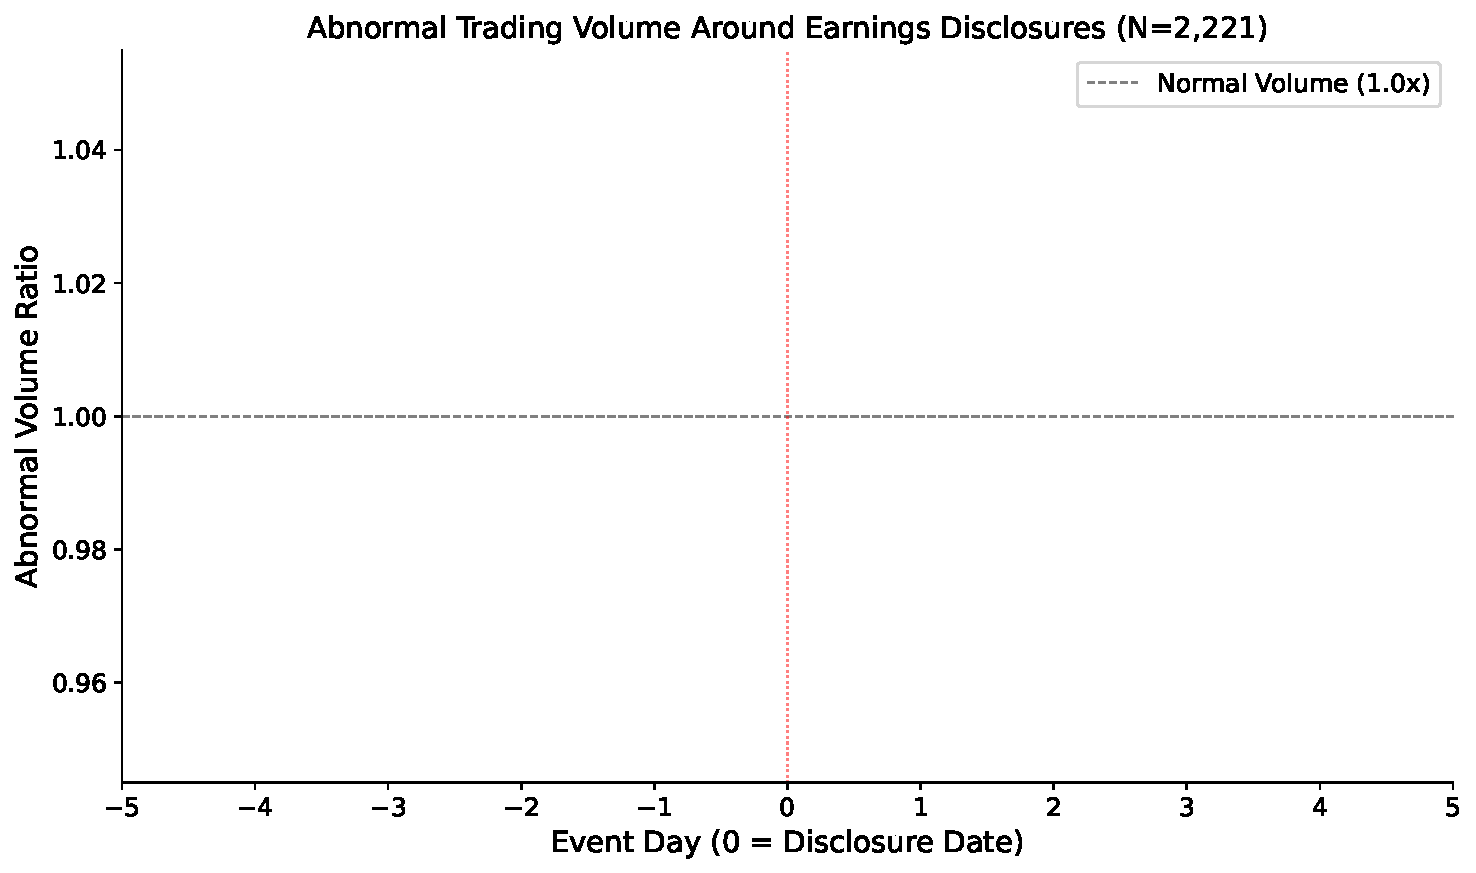
\includegraphics[width=0.85\columnwidth]{figures/fig2_volume.pdf}
\caption{Abnormal trading volume around earnings disclosures ($N$=2,221).}
\label{fig:volume}
\end{figure}

\subsection{Clustered Standard Errors}

Table~\ref{tab:cluster} reports $t$-statistics under alternative specifications. Under month-clustered standard errors, CAR[-5,$-$1] remains significant ($t$=2.15, $p$=0.032) but CAR[-3,$-$1] becomes marginal ($t$=1.80, $p$=0.072), suggesting some parametric significance is inflated by event clustering.

\begin{table}[h]
\caption{Clustered Standard Errors}
\label{tab:cluster}
\begin{tabular}{lrrrrrr}
\toprule
& \multicolumn{2}{c}{Standard} & \multicolumn{2}{c}{Firm-clustered} & \multicolumn{2}{c}{Month-clustered} \\
\cmidrule(lr){2-3} \cmidrule(lr){4-5} \cmidrule(lr){6-7}
Window & $t$ & $p$ & $t$ & $p$ & $t$ & $p$ \\
\midrule
CAR[-5,$-$1] & 4.38 & $<$0.001 & 3.92 & $<$0.001 & 2.15 & 0.032 \\
CAR[-3,$-$1] & 3.47 & $<$0.001 & 2.95 & 0.003 & 1.80 & 0.072 \\
CAR[0,+1] & $-$0.31 & 0.760 & $-$0.25 & 0.802 & $-$0.18 & 0.861 \\
\bottomrule
\end{tabular}
\end{table}

\subsection{Selection Bias Assessment}

Our surprise analysis relies on 584 parseable events (26.4\%). Pre-disclosure CARs are not significantly different between parseable and non-parseable groups (CAR[-3,$-$1]: $p$=0.147). However, parseable events come from larger firms with lower beta, so our surprise-direction results apply primarily to larger chaebol affiliates.

\subsection{Temporal Heterogeneity}

We observe a structural shift in event-day CARs: positive during 2020--2022 (COVID-19 recovery) and negative during 2024--2026. A significant quarterly pattern emerges, with Q1 disclosures generating negative CARs ($-$0.51\%, $p$=0.010) and Q2 generating positive CARs (+0.60\%, $p$=0.003). Cross-sectional OLS of CAR[-3,$-$1] on log(size) and beta yields $R^2=0.002$, confirming that firm characteristics explain virtually none of the pre-disclosure drift.

\begin{figure}[h]
\centering
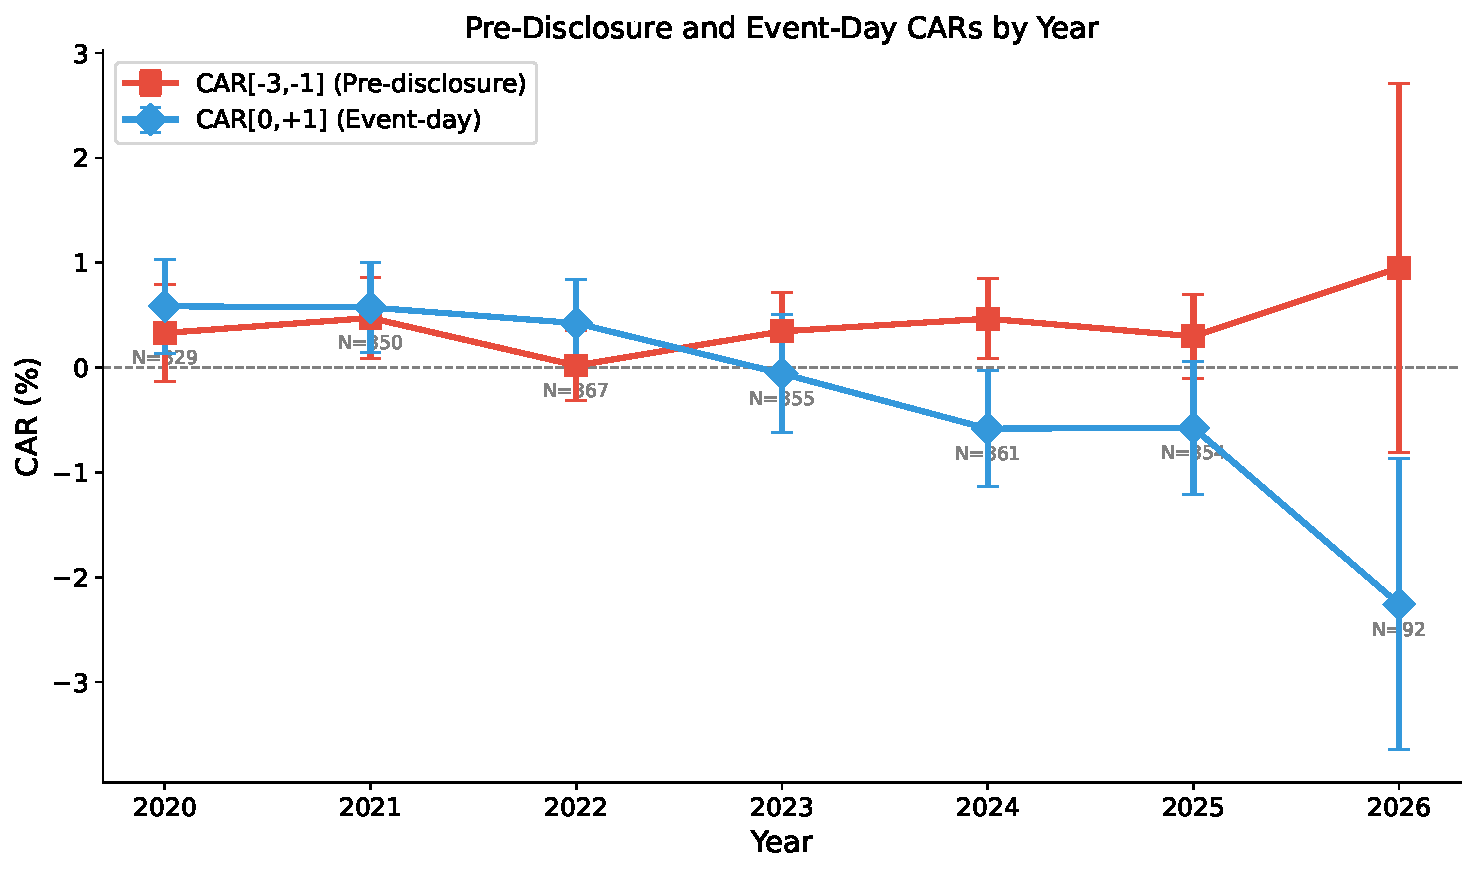
\includegraphics[width=0.85\columnwidth]{figures/fig3_year.pdf}
\caption{Pre-disclosure CAR[-3,$-$1] and event-day CAR[0,+1] by year.}
\label{fig:year}
\end{figure}

\section{Discussion}

\subsection{Drift Without Directional Leakage}

Three complementary tests suggest the drift is non-directional: (1) direction test: 49.0\% accuracy; (2) non-parametric tests: sign test and Wilcoxon fail; (3) surprise conditioning: $p$=0.703. The drift appears driven by company-specific news unrelated to earnings, market momentum, or anticipatory trading based on publicly available signals. This interpretation is consistent with \citet{hirshleifer2003limited}, who argue that limited investor attention can produce predictable patterns without implying illegal information access.

\subsection{Comparison with International Evidence}

Our findings align with the broader evidence on fair disclosure regulation. \citet{bailey2003regulation} find that Reg FD reduced selective disclosure, and \citet{eleswarapu2004impact} document reduced information asymmetry. Our contribution is distinct: we test whether the regulation continues to be effective \textit{within} the regulated regime by examining directional content.

\subsection{Implications}

For regulators, non-directional drift suggests Korea's Fair Disclosure regime does not require fundamental reform. For investors, post-disclosure Day~+1 returns correctly price surprises with 60.6\% accuracy, while pre-disclosure drift strategies are unlikely to be profitable directionally.

\subsection{Limitations}

Our YoY surprise measure is crude; only 26.4\% of events are parseable. The sample is limited to large chaebol affiliates. Korean Fama-French factors are unavailable. We cannot rule out that volume increases reflect legal mosaic information assembly.

\section{Conclusion}

This study finds no evidence of directional information leakage in Korean earnings announcements. Three analyses---direction prediction (49.0\% accuracy), non-parametric tests (sign test $p$=0.585), and surprise conditioning ($p$=0.703)---demonstrate that pre-disclosure drift is non-directional. The first post-disclosure trading day shows strong directional response (60.6\% accuracy, $p$<0.001), consistent with effective fair disclosure.

Our results carry a broader methodological lesson: pre-announcement drift should not be conflated with information leakage without conditioning on the direction of the actual news \cite{meulbroek1992comparison, bernile2016can, atiase1985predisclosure}. Future work should examine non-chaebol firms and incorporate analyst consensus surprises.

\begin{acks}
The author thanks the DART electronic disclosure system for providing publicly accessible corporate filing data. All disclosure data are publicly available through DART (\url{https://dart.fss.or.kr}). Stock price data are from KRX via FinanceDataReader. Analysis code is available at \url{https://github.com/yjkim0123/pre-disclosure-leakage}.
\end{acks}

\bibliographystyle{ACM-Reference-Format}
\bibliography{refs}

\end{document}
